Suppose we have generated a test input that has caused invalid observations of
the SUT.  The generated counterexample consists of (1) {\em signal} that is
essential to triggering violations, and (2) {\em noise} that does not contribute
to revealing such violations.  We need to shrink the counterexample by removing
the noise and keeping the signal.

For interactive testing, the test input is a sequence of request messages.  An
intuitive way of shrinking is to remove some requests from the original sequence
and rerun the test.  However, rerunning an interesting request might produce
trivial results, due to inter-execution nondeterminism discussed in
\autoref{sec:inter-execution}.

To prevent turning signal into noise when rerunning the test, I shrink the
heuristics instead of shrinking the generated test input.
\autoref{sec:shrink-architecture} introduces the architecture for interactive
shrinking, then \autoref{sec:shrink-ir} explains the language design beneath
that addresses inter-execution nondeterminism.

\subsection{Architecture}
\label{sec:shrink-architecture}

I propose a generic framework for generating and shrinking interactive tests.
The key idea is to introduce an abstract representation for test inputs that
embeds trace-based heuristics.  When shrinking the counterexample, the test
harness picks a substructure of the abstract representation and computes the
corresponding test input using the new runtime trace.

For example, when generating a timestamp, instead of producing the concrete
value, \eg, ``\httpdate\today~\currenttime~GMT'', the generator returns an
abstract representation that says, ``use the timestamp observed in the last
response''.  When rerunning the test, the timestamp is computed from the new
trace, \eg, ``\httpdate\DayAfter~\currenttime~GMT''.

\begin{figure}
  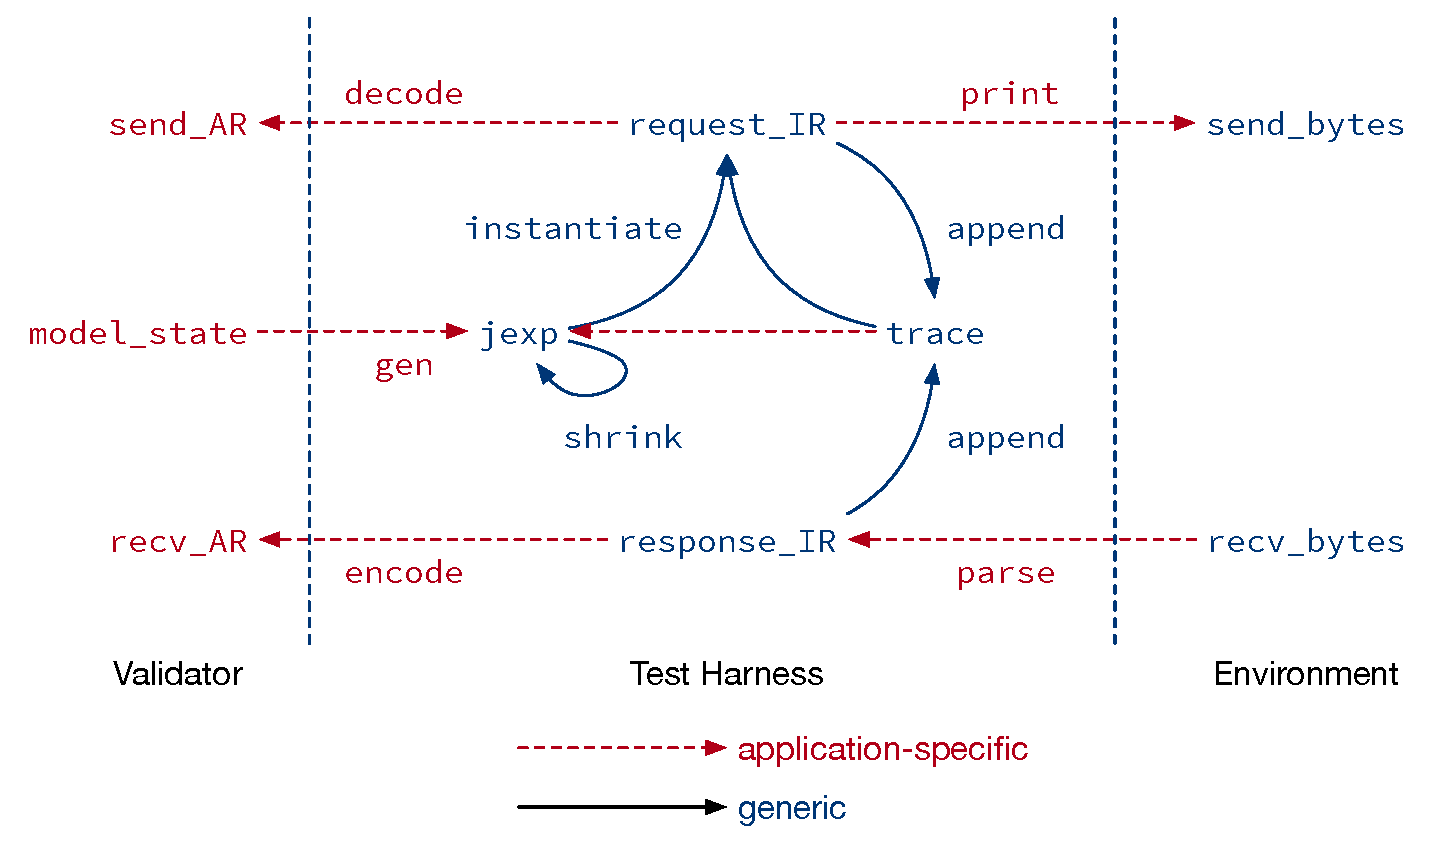
\includegraphics[width=.85\textwidth]{figures/shrink}
  \caption{Complete architecture of the test harness.}
  \label{fig:shrink}
\end{figure}

The test generation and shrinking framework is shown in \autoref{fig:shrink}.
It involves four languages, from right to left:
\begin{enumerate}
  \item Byte representation, in which the tester interacts with the environment.
    This can be network packets, file contents, or other serialized data
    produced and observed by the tester.

  \item Intermediate representation (IR), a generic language that abstracts the
    byte representation as structured data.  The test harness {\em parses} byte
    observations and records its trace in terms of the IR, which allows
    representing trace-based heuristics as a generic language, \ie,
    J-expressions.

  \item J-expression (Jexp), a symbolic abstraction of the IR.  The IR
    corresponds to concrete inputs and outputs, whereas Jexp defines a
    computation from trace to IR.  The generator provides test inputs in terms
    of Jexps; The test harness {\em instantiates} the generated Jexps into
    request IR and {\em prints} them into byte representation.

    When shrinking test inputs, the test harness shrinks the sequence of Jexps.
    The shrunk Jexps are then instantiated by the new trace during runtime.

    The intermediate representation and J-expression will be further explained
    in \autoref{sec:shrink-ir}.

  \item Application representation (AR), including the request (\ilc Q),
    response (\ilc A), and state (\ilc S) types used for specifying the
    protocol.  Specification writers can choose the type interface at their
    convenience, provided the request and response types are embeddable into the
    IR.
\end{enumerate}

The testing framework implements protocol-independent mechanisms like recording
the trace and shrinking counterexamples, which correspond to the blue solid
arrows in \autoref{fig:shrink}.  It can be used for testing various protocols,
provided application-specific translations from IR to AR and between IR and
bytes, illustrated as red dotted arrows.  The test developer needs to tune the
generator that produces Jexps, encoding their domain knowledge as state-based
and trace-based heuristics.

\subsection{Abstract representation languages}
\label{sec:shrink-ir}
I choose JSON as the IR in this framework, which allows syntax trees to be
arbitrarily wide and deep and provides sufficient expressiveness for encoding
message data types in general.

\begin{figure}
\[\begin{array}{r@{\;}l}
\mathsf{JSON^T}\triangleq&\mathsf T\mid\{\mathsf{object^T}\}\mid[\mathsf{array^T}]\mid\mathsf{string}\mid\Int\mid\Bool\mid\mathsf{null}\\
\mathsf{object^T}\triangleq&\nil\mid\mathsf{``string": JSON^T,object^T}\\
\mathsf{array^T}\triangleq&\nil\mid\mathsf{JSON^T,array^T}\\
\mathsf{IR}\triangleq&\mathsf{JSON^{IR}}\\
\mathsf{Jexp}\triangleq&\mathsf{JSON^{\Jref{\Label}{\Jpath}{\Function}}}\\
&\text{where }\Label\in\Nat,\Function\in\mathsf{IR}\to\mathsf{IR}\\
\Jpath\triangleq&\This\mid\Jpath\Number\Index\mid\Jpath\At\Field\\
&\text{where }\Index\in\Nat,\Field\in\mathsf{string}
\end{array}\]
\caption{Intermediate representation and J-expression.}
\label{fig:ir-jexp}
\end{figure}

\begin{figure}
\begin{minipage}{.6\textwidth}
\begin{coq}
Notation   labelT := nat.
Definition traceT := list (labelT * IR).

Context q1 q2 a1 a2 : IR.
Example labelled_trace: traceT :=
  [(1, q1); (3, q2); (4, a2); (2, a1)].
\end{coq}
\end{minipage}\begin{minipage}{.3\textwidth}
  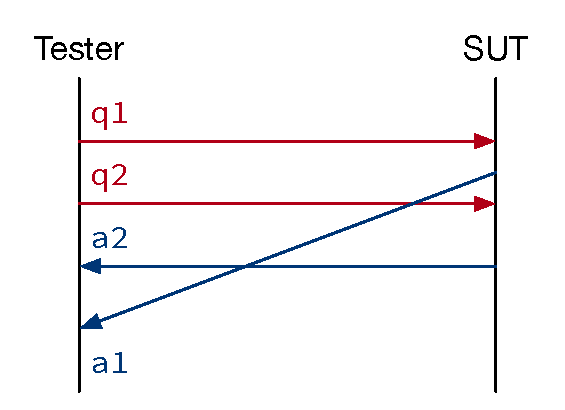
\includegraphics[width=\linewidth]{figures/ir-trace}
\end{minipage}
\caption{Labelled trace example.}
\label{fig:ir-trace}
\end{figure}

\begin{figure}
  \begin{minipage}[t]{.4\textwidth}
\begin{json}
  (* a2 = *)
  {
    "files": [
      {
        "name": "foo",
        "mode": 755
      },
      {
        "name": "bar",
        "mode": 500
      }
    ],
    "exitCode": 0
  }
\end{json}
  \end{minipage}\begin{minipage}[t]{.5\textwidth}
\begin{coq}
(* Jpath syntax defined in %\autoref{fig:ir-jexp}%. *)
Example second_file_mode: jpath :=
  this @ "files" # 2 @ "mode".

Example mode_add_write (j: IR) : IR :=
  match j with
  | JSON_Number n =>
    JSON_Number (mode_bits_or 200 n)
  | _ => j
  end.

Example id (j: IR) : IR := j.
\end{coq}
  \end{minipage}
\vspace*{1em}
  \caption{IR, Jpath, and heuristics function example.}
  \label{fig:ir-jpath}
\end{figure}

\paragraph{Syntax}
The J-expression is an extension of JSON that can encode trace-based heuristics.
As shown in \autoref{fig:ir-jexp}, a Jexp may include syntax
$(\Label.\Jpath.\Function)$ that represents trace-based heuristics, specified as:
\begin{enumerate}
\item The test harness records the trace as a list of labelled messages, where
  the requests are labelled odd, and their responses are labelled as the next
  even number.  The $\Label$ in a Jexp locates the IR in the trace with which
  the heuristics computes the input.  Labelling messages allows the reproducing
  trace-based heuristics despite shrinking and inter-execution nondeterminism.

  For example, consider the trace in \autoref{fig:ir-trace}: If a trace-based
  heuristics is interested in \ilc{q2}'s response \ilc{a2}, then it can be
  encoded as ``compute the test input based on message labelled 4'':
\begin{coq}
  Context get_label: labelT -> traceT -> IR.

  Compute get_label 4 labelled_trace.
  (* = a2 : IR *)
\end{coq}
  
  Suppose the test input is shrunk by removing \ilc{q1}, the label for \ilc{q2}
  remains unchanged as 3, so label 4 corresponds to the new response to
  \ilc{q2}:
\begin{coq}
  Example new_trace: traceT :=
    [(3, q2); (4, a2')].

  Compute get_label 4 new_trace.
  (* = a2' : IR *)
\end{coq}

As a result, the trace-based heuristics are preserved and adapted to new
executions during the shrinking process.
\item The $\Jpath$ is a path in the IR's syntax tree and refers to a
  substructure of the IR that the heuristics uses.

  For example, suppose request \ilc{q2} lists files in a directory using the
  POSIX \inlinec{ls} command, and its response \ilc{a2} is encoded as the IR
  shown in \autoref{fig:ir-jpath}.  The response IR is a JSON object whose
  \inlinec{"files"} field is an array of objects, each has a \inlinec{"name"}
  and a \inlinec{"mode"} field.  A heuristic can refer to the second file's
  mode bits by Jpath \ilj{(this@"files"#2@"mode")}, which will guide the test
  harness to locate its corresponding value:
\begin{coq}
  Context get_jpath: jpath -> IR -> IR.

  Compute get_jpath second_file_mode a2.
  (* = JSON_Number 500 : IR *)
\end{coq}
\item The $\Function$ has type $(\mathsf{IR}\to\mathsf{IR})$, and defines the
  computation based on the sub-IR located by the Jpath.

  Consider the mode bits located in the previous example: If the heuristic
  wants to add write permission to the mode bits, it can do so with the
  \ilc{mode_add_write} function in \autoref{fig:ir-jpath}, which produces mode
  700.  Some heuristics might use the sub-IR 500 as-is, using the identity
  function \ilc{id}.
\end{enumerate}

\paragraph{Semantics}
J-expression provides a generic interface for test developers to implement
trace-based heuristics.  For the aforementioned file system example, the tester
can generate a request that changes the mode bits of an observed file, with the
following Jexp:
\begin{json}
  (* e5 = *)
  {
    "command": "chmod",
    "args":
      [ 4.(this@"files"#2@"mode").mode_add_write
      , 4.(this@"files"#2@"name").id ]
  }
\end{json}

To instantiate Jexps into request IR, the test harness substitutes all
occurences of $(\Jref{l}{p}{f})$ in the Jexp with its corresponding IR computed
from the runtime trace:
\begin{coq}
  Definition eval (l: labelT) (p: jpath) (f: IR -> IR) (t: traceT) : IR :=
    let a: IR := get_label l t in
    let j: IR := get_jpath p a in
    f j.
\end{coq}

For example, given the runtime trace in \autoref{fig:ir-trace}, with \ilc{a2} is
defined in \autoref{fig:ir-jexp}, the the above Jexp is instantiated into the
following request:

\begin{json}
  (* instantiate e5 labelled_trace = *)
  { 
    "command": "chmod",
    "args": [ 700, "bar" ]
  }
\end{json}

However, when rerunning the test, the \ilc{new_trace} has a different response
associated with label 4.  The new response \ilc{a2'} might have fewer than 2
files in its payload.  Moreover, the response \ilc{a2'} might have not appeared
in the trace, due to delays in the environment.

To instantiate the original Jexp in such situations, I loosen the
\ilc{get_jpath} and \ilc{get_label} functions when evaluating the heuristics:
\begin{enumerate}
\item When evaluating a Jpath starting with \ilj{p#n}, if \ilj p corresponds to
  an array with fewer than \ilj n elements, or the array's \ilj n-th element
  cannot properly evaluate the remaining path, then try continuing the
  evaluation with any other element in the array.

  For example, consider evaluating \ilj{(this@3#"bar")} on the following IR's:
  \begin{multicols}{2}
\begin{json}
  (* j2 = *)
  [
    { "foo": 21 },
    { "bar": 22 }
  ]
\end{json}
\columnbreak
\begin{json}
  (* j3 = *)
  [
    { "bar": 31 },
    { "baz": 32 },
    { "foo": 33 }
  ]
\end{json}
  \end{multicols}

  Here \ilj{j2} doesn't have a third element, and \ilj{j3}'s third element
  doesn't have field \ilj{"bar"}.  In these cases, \ilj{get_jpath} chooses other
  elements in the two arrays, resulting in value \ilj{22} for \ilj{j2}, and
  \ilj{31} for \ilj{j3}.
  
\item When evaluating label \ilj l and Jpath \ilj p on a trace, if the message
  labelled \ilj l does not exist in the trace, or cannot evaluate Jpath \ilj p
  properly, then try continuing the evaluation with any other IR in the trace.

  For example, consider evaluating J-expression \ilj{6.(this#2@"foo").id} on the
  following traces:
\begin{coq}
  Definition t1: traceT :=
    [(1,q1); (2,j2); (5,q2)].

  Definition t2: traceT :=
    [(3,q1); (4,j3); (5,q2); (6,a2)].
\end{coq}

Here \ilj{t1} doesn't have a message labelled 6, probably caused by environment
delays; \ilj{t2} has label 6 but its corresponding message is an object rather
than an array expected by the Jexp.  In these cases, \ilc{eval} chooses other
messages in the trace to evaluate, resulting in value \ilc{21} for \ilc{t1}, and
\ilc{33} for \ilc{t2}.
\end{enumerate}

By introducing loose evaluation of J-expressions, my test harness allows partial
instantiation of heuristics when the runtime trace is less than satisfying.

So far I have shown how to generate and shrink interactive test inputs and
address inter-execution nondeterminism.  In the next chapter, I'll combine this
test harness design with the validator practice in \autoref{chap:practices}, and
evaluate these techniques by testing real-world systems like HTTP servers and
file synchronizers.
